
%\documentclass[11pt, notes]{beamer}       % print frame + notes
%\documentclass[notes=only]{beamer}   % only notes
%\documentclass[10pt]{beamer}              % only frames

%\documentclass[aspectratio=169, 10pt, notes]{beamer}
%\documentclass[aspectratio=169, 10pt, handout, notes]{beamer}
\documentclass[aspectratio=169, 10pt, handout]{beamer}

\usepackage{booktabs}
\usepackage{color}
\usepackage{ulem}
\usepackage{hyperref}
\usepackage{sidecap}
\usepackage{epstopdf}
\usepackage{enumerate}
\usepackage{bbm}
\usepackage{caption}
\usepackage{subfigure}
\usepackage{subfig}
\usepackage{multicol}
\usepackage{lmodern}
\usepackage{lipsum}
\usepackage{marvosym}
\usepackage{booktabs}
\usepackage{changepage}
\usepackage{natbib}
\usepackage{eurosym}
\usepackage{cancel}
\usepackage{pifont}


\newcommand{\backupbegin}{
   \newcounter{framenumberappendix}
   \setcounter{framenumberappendix}{\value{framenumber}}
}
\newcommand{\backupend}{
   \addtocounter{framenumberappendix}{-\value{framenumber}}
   \addtocounter{framenumber}{\value{framenumberappendix}} 
}

\newenvironment{wideitemize}{\itemize\addtolength{\itemsep}{10pt}}{\enditemize}


\DeclareOptionBeamer{compress}{\beamer@compresstrue}
\ProcessOptionsBeamer

\mode<presentation>

\useoutertheme[subsection=false,shadow]{miniframes}
\useinnertheme{circles}

\beamertemplatenavigationsymbolsempty

\setbeamertemplate{footline}[frame number]

\begin{document}

\title{Behavioral Development Economics}
\subtitle{Chapter prepared for the Handbook of Behavioral Economics (Vol 2)}

%\setbeamertemplate{footline}[page number]


\author{Michael Kremer (Harvard and NBER) \quad \quad \quad \quad Gautam Rao (Harvard and NBER)\\ 
\vspace{1cm}
Frank Schilbach (MIT and NBER)}
\date{February 2019}


%TITLE FRAME
%%%%%%%%%%%%%%%%%%%%%%%%%%%%%%%%%%
\begin{frame}
%%%%%%%%%%%%%%%%%%%%%%%%%%%%%%%%%%
  \titlepage
  
  \note{
  
  \begin{itemize}
  
    	\item This is joint work by Michael Kremer (Harvard), Gautam  Rao (Harvard) and Frank Schilbach (MIT) in the forthcoming Handbook of Behavioral Economics. We thank Xinyue Lin and Fanele Mashwama for excellent Research Assistance. 

    \end{itemize}

}
    
\end{frame}

%%%%%%%%%%%%%%%%%%%%%%%%%%%%%%%%%%
\section{1 Intro}
%%%%%%%%%%%%%%%%%%%%%%%%%%%%%%%%%%

%%%%%%%%%%%%%%%%%%%%%%%%%%%%%%%%%%
\begin{frame}{The rise of behavioral development economics}
%%%%%%%%%%%%%%%%%%%%%%%%%%%%%%%%%%

\begin{wideitemize}

	\item \textbf{Historical views of development:} People were thought to be very different before and after the advent of ``modernity". e.g.\:

	\begin{itemize}

		\item Pre-capitalist vs.\ capitalist \citep{marx1967communist} 
		
		\item Tradition vs.\ rationalism (Weber and Durkheim)
        
		\item Mechanical vs.\ organic solidarity

		\item Modernization theory: modernization as a process of radical social change but also change in ways of thinking and seeing the world
	
	\end{itemize}

	\item \textbf{Development economics:} emerged as a critical response to this view.

	\begin{itemize}

		\item Sees farmers as essentially rational capitalists (but maybe facing market failures)
	
		\item Rejects seemingly non-falsifiable cultural explanations (e.g.\ ``Hindu rate of growth") 

	\end{itemize}


\end{wideitemize}

\note{
  
\begin{itemize}
  
    \footnotesize
  
    \item Historically, writers on process that we now call development believed that people thought very differently before and after rise of modernity. These differences can be seen in the way writers wrote about.

    \item Notes on modernization theory:
    \begin{itemize}
    
        \scriptsize
    
        \item More secular, more democratic, more politically stable, more division of labor.
        \item Relationships in rich countries are less multi-stranded (e.g. landlord and creditor and political representative), 
        \item Rich countries have more inter-generational social mobility; ideology of equality rather than hierarchy.
        \item More rule of law rather than personalistic rules.
        \item More geographic mobility; more openness to jobs across gender

        \item Assignment of jobs by educational qualifications
        \item More nuclear family
    \end{itemize}

    \item Idea of modernization theory is institutional structures and institutional activities become more highly specialized, differentiated, and integrated.

    \item Urbanization literacy, bureaucracy, mass media, society becomes more participatory, development of political parties, civil service, bureaucracy

    \item Move from relations based on tradition and loyalty to those based on rational exchange

    \item People more future oriented, treatment oriented, and concerned with rights of individuals; less fatalistic.

    \end{itemize}

}

\end{frame}

%%%%%%%%%%%%%%%%%%%%%%%%%%%%%%%%%%
\begin{frame}{The rise of behavioral development economics (cont'd)}
%%%%%%%%%%%%%%%%%%%%%%%%%%%%%%%%%%

\begin{wideitemize}

	\item The dominant view in development economics up to about the 1990s is that the poor are ``poor but efficient" \citep{schultz1964transforming}
	
	\item This view started to change during the past two decades.
	
	\begin{itemize}
	
		\item With rise of behavioral economics, a more psychologically realistic view of human behavior has entered development economics
		
		\item Systematic deviations from standard models in preferences, beliefs, and decision-making

		\item So far, relies mostly on ``universal" insights from psychology about human behavior
		
		\item Some attention to differences in psychology across cultures or across rich and poor

		\item Studies of the interaction of behavioral biases with the institutions and markets specific to developing economies.

	\end{itemize}
	
\end{wideitemize}

\end{frame}

%%%%%%%%%%%%%%%%%%%%%%%%%%%%%%%%%%
\begin{frame}{Caveats and critiques of behavioral development economics}
%%%%%%%%%%%%%%%%%%%%%%%%%%%%%%%%%%

\noindent Behavioral development economics...

\bigskip

\begin{wideitemize}

	\item[(1)] Attempts to augment and improve, and not supplant, existing models. 
	
	\item[(2)] Does not deny the importance of institutions for development 
	
	\item[(3)] Is sometimes critiqued for dismissing real incentives and constraints that apparently ``irrational" actions reflect (e.g.\ \cite{rosenzweig2014rainfall})
	The best research in this subfield overcomes this challenge by testing specific behavioral mechanisms rather than simply identifying an apparent failure of the standard model.

	
\end{wideitemize}

\note{

\begin{itemize}
    
    \item Prices and incentives still matter!
    
    \item Behavioral models attempt to parsimoniously capture important aspects of psychology
    
    \item As opposed to generically labelling any residual in a rational model as behavioral

\end{itemize}

}

\end{frame}

%%%%%%%%%%%%%%%%%%%%%%%%%%%%%%%%%%
\begin{frame}{Caveats and critiques of behavioral development economics (cont'd)}
%%%%%%%%%%%%%%%%%%%%%%%%%%%%%%%%%%

\noindent Behavioral development economics...

\bigskip

\begin{wideitemize}

	\item[(4)] Does not ``blame the poor" for their poverty since it is (i) typically concerned with universal psychological factors and (ii) does not stipulate that behavioral biases are blameworthy.
	
	\item[(5)] Critique that behavioral econ proposes paternalistic policies that restrict individual choices. There is truth to this critique. But weigh this concern against bad policy outcomes  that can result from misunderstanding human behavior. 
	
	\item[(6)] Occasionally rejects robust lab-experimental results which are found to be less important in the real world (e.g.\ \cite{cohen2010free}; \cite{ashraf2010can})

\end{wideitemize}

\note{

\begin{itemize}
    
    \item Regarding (5): 
        \begin{itemize}
        \item some arguments for libertarian paternalism (e.g.\ Thaler and Sunstein 2003) -- help behavioral agents while not distorting choices by individuals who are fully optimizing already (e.g.\ by setting defaults).
    
    
        \item In fact, the subtleties concerning welfare in a behavioural world generally call for humility on the part of the policy maker; see paper for more
        \end{itemize}
    \item Regarding (6):
        \begin{itemize}
            \item For example, some have conjectured that reducing the cost of preventive health products such as mosquito nets or distributing them for free would lead people to value them less and use them less.
    
            \item Rigorous testing by \cite{cohen2010free} and \cite{ashraf2010can} yields no support for this conjecture. Broadly speaking, this evidence has moved the policy debate towards free distribution of preventive health goods such as mosquito nets
        \end{itemize}
    
\end{itemize}

}

\end{frame}


%%%%%%%%%%%%%%%%%%%%%%%%%%%%%%%%%%
\begin{frame}{Topics covered (organized by behavioral concepts)}
%%%%%%%%%%%%%%%%%%%%%%%%%%%%%%%%%%

\begin{itemize}

	\item \textbf{Non-standard preferences}

	\begin{itemize}

		\item Time preferences (present bias) 
	
		\item Risk preferences (loss aversion, reference dependence, narrow bracketing)
		
		\item Social preferences

	\end{itemize}
	
	\smallskip
	
	\item \textbf{Non-standard beliefs}
	
	\begin{itemize}

		\item Naivete, projection bias
		
		\item Non-Bayesian learning, redundancy neglect
			
		\item Motivated reasoning

	\end{itemize}
	
		\smallskip

	\item \textbf{Non-standard decision-making}
	
	\begin{itemize}
			
		\item Limited attention and memory
		
		\item Mental accounting
		
		\item Default effects 

    	%\item {Psychology of poverty}

	\end{itemize}


\end{itemize}

\end{frame}


%%%%%%%%%%%%%%%%%%%%%%%%%%%%%%%%%%
\section{2 Euler puzzle}
%%%%%%%%%%%%%%%%%%%%%%%%%%%%%%%%%%


%%%%%%%%%%%%%%%%%%%%%%%%%%%%%%%%%%
\begin{frame}{Topics covered (organized by development economics)}
%%%%%%%%%%%%%%%%%%%%%%%%%%%%%%%%%%

\begin{enumerate}[(1)]

	\small

	\item[(1)] Introduction 
	
	\item[(2)] \textbf{High rates of return without rapid growth (Euler equation puzzle)}

	\only<2->{
	
	\begin{enumerate}[(A)]
	
	\footnotesize
		\item Euler Puzzle
		
		\item Present bias
		
		\item Reference-dependent preferences
		
		\item Other behavioral factors (e.g.\ biased beliefs)
	
	\end{enumerate}
	
	}

	\item[(3)] Health
	
	\item[(4)] Savings
	
	\item[(5)] Risk and insurance

	\item[(6)] Technology adoption
	
	\item[(7)] Labor

	\item[(8)] Firms
	
	\item[(9)] Social preferences, culture, and development
	
	\item[(10)] The psychology of poverty

\end{enumerate}

\end{frame}

%%%%%%%%%%%%%%%%%%%%%%%%%%%%%%%%%%
\begin{frame}{High returns to capital in many contexts \cite{banerjee2005growth}}
%%%%%%%%%%%%%%%%%%%%%%%%%%%%%%%%%%

\begin{wideitemize}

	\item Borrowing at very high rates (70 to 100\% annual rates and more)
	
	\begin{itemize}
	
		\item Small-time fruit vendors in Chennai who borrow at daily rates of 5\% \citep{karlan2018debt}
		

	\end{itemize}

	\item High returns to small-business grants \citep{de2008capital}
	
	\item High returns to inventories \citep{kremer2013behavioral}
	
	\item Predictable large increases in prices between seasons \citep{burke2018sell}
	
\end{wideitemize}

\note{
    \begin{itemize}
        \item \cite{karlan2018debt} randomized paying off the loans of fruit vendors in Chennai. These vendors generally managed to stay out of debt for several weeks, but then fell back into debt, generally after a health shock or unexpected expense. Once that happened, they failed to pay off their debt on their own. 
    \end{itemize}

}

\end{frame}

%%%%%%%%%%%%%%%%%%%%%%%%%%%%%%%%%%
\begin{frame}{Euler equation} % , even in absence of any capital market}
%%%%%%%%%%%%%%%%%%%%%%%%%%%%%%%%%%

\begin{wideitemize}

	\item Suppose production function $F(K)$ with $F^{\prime} (K) \geq 0$ and $F^{\prime \prime} (K) \leq 0$.
	
	
	\item Standard Euler equation links consumption growth to marginal return to capital:
	\begin{align}
	u^{\prime} (c_t)= \delta F^{\prime}(K_t) u^{\prime} (c_{t+1})
	\end{align}

	\item Implies (unrealistically) high consumption growth rates.
	
	\begin{itemize}

		\item If log utility, $F^{\prime}(K ) =  50\%$ annually, and $\delta = 0.96$, then  $\frac{\dot{c}}{c} = 44\%$.

		\item If constant intertemporal elasticity of substitution utility with $\sigma = 2$, then $\frac{\dot{c}}{c} = 20\%$. 

		\item Still implies 38-fold consumption growth in 20 years. 
		
	\end{itemize}

	\item Need high ``tax" or discount rate to resolve puzzle.
		
	\begin{itemize}
	    
	    \item Implicit taxes due to corruption or redistributive pressures by from extended family members
	    
	    \item Allowing for realistic values of such taxes does not resolve puzzle (\cite{jakiela2015does}).
	    
	\end{itemize}

\end{wideitemize}




\end{frame}

%%%%%%%%%%%%%%%%%%%%%%%%%%%%%%%%%%
\begin{frame}{Puzzle persists even with non-concave production function.} % , even in absence of any capital market}
%%%%%%%%%%%%%%%%%%%%%%%%%%%%%%%%%%

\begin{wideitemize}

	\item Non-concave production functions are a feature of poverty trap models.
	
	\begin{itemize}
	
		\item Implies multiple steady-states and sustained poverty below threshold level

	\end{itemize}
	
	\item But observed initial conditions need to be consistent with model.
	
	\begin{itemize}
	
		\item Steady state will have low rate of return.
		
		\item Euler equation will be satisfied (FOC).
		
		\item Individuals with high rate of return should have fast consumption growth.
	
	\end{itemize}
	
	\item Poverty trap models also suggest a transformative effect of credit.

	\begin{itemize}

		\item Seems counterfactual: limited uptake, limited transformation \citep{banerjee2015microcred,meager2018understanding}
		
	\end{itemize}


\end{wideitemize}

\end{frame}

%%%%%%%%%%%%%%%%%%%%%%%%%%%%%%%%%%
\begin{frame}{Stochastic income and risk aversion?} % , even in absence of any capital market}
%%%%%%%%%%%%%%%%%%%%%%%%%%%%%%%%%%

\begin{itemize}

	\item Maybe people don't invest because investments (e.g.\ fertilizer) are risky? Suppose income in period $t$ is:
	\begin{align}
	Y_{t} = Y_0 + \epsilon_t + \sum_{i=1}^n \mu_{i,t}  F_i(K_{i,t}),
	\end{align}
	
	where $n$ assets/capital goods, arbitrary pattern of correlation. 
	
	\bigskip
	
	\item Stochastic Euler equations:
  	\begin{align}
	u^{\prime}(c_t) = \delta \mathbbm{E}_t [ \mu_{i,t}  F_i^{\prime} (K_{i,t}) u^\prime (c_{t+1})], \quad i=1, 2 ,..., n
  	\end{align}

	\item Given initial capital stock, risk aversion will:
	
	\begin{itemize}
	
		\item[(i)] reduce investment in assets which co-vary positively with consumption

		\item[(ii)] increase investment in assets which co-vary negatively with consumption

	\end{itemize}
	
\note{
    \begin{itemize}
        \item This allows for arbitrary correlation between the $\mu$ and $\epsilon$.
        \item $F$ function gives the value of the output in the next period including any remaining value of the capital.
    \end{itemize}

}
	
%	\bigskip 

%	\item But...


\end{itemize}

\end{frame}

%%%%%%%%%%%%%%%%%%%%%%%%%%%%%%%%%%
\begin{frame}{But: Optimal to build buffer stock savings \citep{deaton1991saving,carroll1997buffer}.}
%%%%%%%%%%%%%%%%%%%%%%%%%%%%%%%%%%

\begin{wideitemize}
	
	\item If patient, risk averse, and subject to large shocks, agents want to accumulate large buffer stock savings. 
	
	\begin{itemize}

    	\item At any one time, only a few people should have low buffer stock.
	
	\end{itemize}

	\item For majority with  large buffer stock, consumption should not move much with:

	\begin{itemize}

		\item high-frequency income shocks
		
		\item predictable income changes (e.g.\ seasons)

	\end{itemize}

	\item Implies that even if returns to fertilizer highly correlated with income in season, only modestly correlated with lifetime income and thus consumption

	\begin{itemize}
		
		\item Beta of fertilizer investment (correlation of return with overall consumption) will be modest, and risk aversion will only modestly reduce fertilizer investment

	\end{itemize}

\end{wideitemize}

\end{frame}


%%%%%%%%%%%%%%%%%%%%%%%%%%%%%%%%%%
\begin{frame}{Model with patient consumers seems to make incorrect predictions.}
%%%%%%%%%%%%%%%%%%%%%%%%%%%%%%%%%%

\begin{wideitemize}

	\item In reality:

	\begin{itemize}
	
		\item Liquid buffer stocks are often modest \citep{deaton1991saving}.
	
		\item Consumption co-varies with income, including predictable income \citep{townsend1995consumption}.
	
		\item \cite{karlan2014agricultural} find that rainfall insurance increases fertilizer use.

	\end{itemize}
	
	\item A model will impatient agents can create these predictions.

	\item Thus with either deterministic or stochastic Euler equation, matching the data requires a high effective discount rate.

\end{wideitemize}


\end{frame}

%%%%%%%%%%%%%%%%%%%%%%%%%%%%%%%%%%
\begin{frame}{High discount rates?}
%%%%%%%%%%%%%%%%%%%%%%%%%%%%%%%%%%

\begin{wideitemize}

	\item Maybe $\delta = 50\%$?
	
	\item Standard exponential discounting model has only one parameter for all time horizons.
	
	\begin{itemize}
	
	    \item Euler equation typically considers short horizons ($\leq 1$ year).
    
        \item In exponential discounting model, high short-run discount rate implies that distant future is discounted at extremely high rates.

	    
	\end{itemize}

    \item Absurd implications

	\begin{itemize}

		\item $\delta = 0.5$ implies would not give up \$1 today for \$1 billion in 30 years.
		
		\item No one would own land, get an education, etc.

	\end{itemize}	

\end{wideitemize}

\end{frame}

%%%%%%%%%%%%%%%%%%%%%%%%%%%%%%%%%%
\begin{frame}{Quasi-hyperbolic discounting (present bias)?}
%%%%%%%%%%%%%%%%%%%%%%%%%%%%%%%%%%

\begin{columns}[T] % align columns

\begin{column}{.43\textwidth}
  
\vspace{0.4cm}

\begin{wideitemize}

	\item Alternative hypothesis: present bias ($\beta, \delta$,  \cite{laibson1997golden}))
	
	\begin{itemize}
	
		\item High discount rate between now and tomorrow

		\item Low discount rate between future periods

	\end{itemize}
	
	\pause
	
	\item Can generate both high short-run discounting \textit{and} relatively high long-run patience.

\end{wideitemize}

\end{column}%

\begin{column}{.63\textwidth}
\resizebox{\textwidth}{!}{
\vspace{7cm} 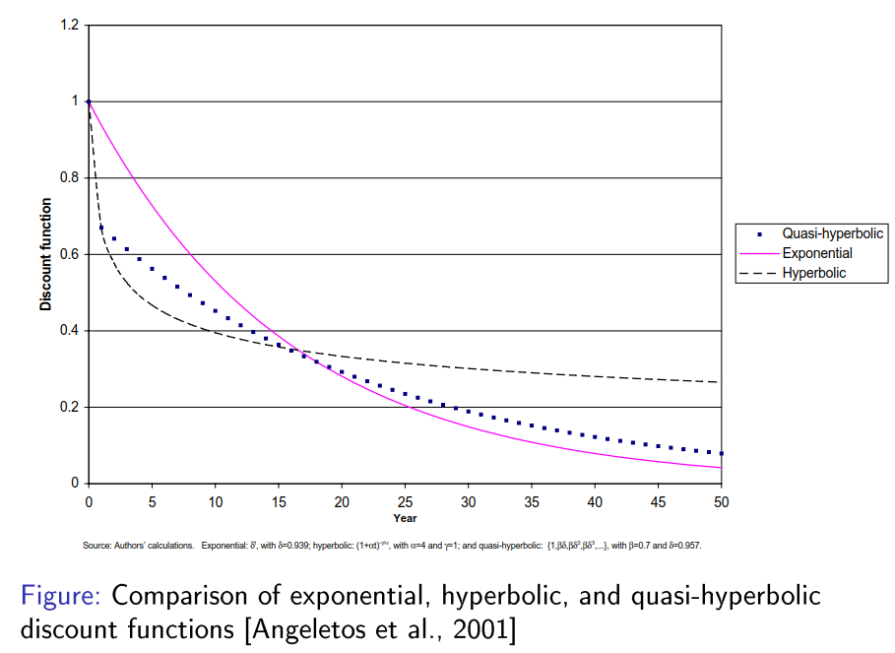
\includegraphics{Picture1.png} 
}
\end{column}%
\hfill%

\end{columns}

\note{
    \begin{itemize}
        \item This is consistent with large experimental literature, literature on developed economics 
        
        \item With reasonably calibrated parameters, present biased person will often care more about the distant future than exponential discounter
        
        \item Note that there is limited evidence in behavioral economics on whether hyperbolic or quasi-hyperbolic discounting is the more accurate model. But lots of evidence against constant discounting from the lab and from field data.
    \end{itemize}
}
\end{frame}



%%%%%%%%%%%%%%%%%%%%%%%%%%%%%%%%%%
\begin{frame}{Implications of present-biased preferences}
%%%%%%%%%%%%%%%%%%%%%%%%%%%%%%%%%%

\begin{wideitemize}
	
	\item Predictions behavior of present-biased agents \citep{angeletos2001hyperbolic}:
	
	\begin{itemize}

		\item Rapidly spend down liquid assets, becoming effectively liquidity constrained
	
		\item Build up (or hold) a stock of illiquid assets that pay off in distant future
	
		\item Leave high rate of return investments on the table, if effectively liquidity constrained

		\item Not be able to smooth consumption; consumption will co-move with income shocks, even with predictable income variation

	\end{itemize}

	\item The sophistication of the present biased actor will determine the degree of procrastination and demand for commitment devices \citep{o1999doing,ODonoghue2001}.
	
	\item Implies modified Euler equation \citep{harris2001dynamic}
	
\end{wideitemize}

\end{frame}

%%%%%%%%%%%%%%%%%%%%%%%%%%%%%%%%%%
\begin{frame}{Methodological aside: Measuring time preferences}
%%%%%%%%%%%%%%%%%%%%%%%%%%%%%%%%%%

\begin{wideitemize}

	\item There is no broadly accepted and easily implementable approach to measuring time preferences. See \cite{cohen2016measuring} for excellent review.

	\item Common approaches include:
	
	\begin{wideitemize}
	
		\item[(1)] Providing choices between monetary payments earlier or later in time \citep{andersen2008eliciting,andreoni2012estimating}. But choices over money may not reveal time preferences since MPC not equal to 1.
		
		\item[(2)] Providing choices between consumption events and effort \citep{mcclure2007time,augenblick2015working}. But consumption outside the experiment might adjust in response. These methods are also likely to be logistically more challenging. 
		
        \item[(3)] Non-incentivized survey measures \citep{falk2018global}.

	\end{wideitemize}

    \item Often trade-off between ease of implementation and mapping into conceptual framework. 


\end{wideitemize}

\note{
    \begin{itemize}
    
        \item If measuring time preferences is central to the research, implementing a real-effort task as in \cite{augenblick2015working} or \cite{augenblick2018short} may be the best option. 
        
        \item If not, utilizing a money earlier-or-later task may still provide some signal of patience over monetary payments, even if it does not cleanly isolate time preferences.

    
    \end{itemize}

}

\end{frame}

%%%%%%%%%%%%%%%%%%%%%%%%%%%%%%%%%%
\begin{frame}{Can loss aversion help explain high expected returns?}
%%%%%%%%%%%%%%%%%%%%%%%%%%%%%%%%%%

\begin{wideitemize}

	\item Experimental evidence suggests that many people are loss averse (rather than risk averse). 
	
	\begin{itemize}

	    \item See review of work on reference-dependent preferences by \cite{o1999doing}.
 
	\end{itemize}
	

	\item Kink in utility function around a reference point; losses felt more strongly than gains \citep{kahneman47l979}.

	\begin{itemize}
	
		\item Empirical estimates that people weigh losses 2-3 times as much as gains: e.g. turn down gambles with equal chance of winning \$2 and losing \$1.
		
		\item With narrow bracketing, loss aversion could inhibit many investments facing farmers and small businesses.

	\end{itemize}

\end{wideitemize}

\end{frame}

%%%%%%%%%%%%%%%%%%%%%%%%%%%%%%%%%%
\begin{frame}{Loss aversion and investment}
%%%%%%%%%%%%%%%%%%%%%%%%%%%%%%%%%%

\begin{wideitemize}

	\item Shopkeepers in Kenya exhibiting greater loss aversion in experimental tasks maintain lower inventories \citep{kremer2013behavioral}.
	
	\item Asset by asset; people may be hesitant to give up existing assets to invest in new assets, making asset allocations sticky, maybe reducing migration.

	\item Under loss aversion, loans collateralized with assets purchased under the loan will have high uptake and low default. (\cite{jack2016borrowing}; \cite{carney2018}).
	
	\item Predicts stickiness of wealth rather than poverty trap:
	
	\begin{itemize}
	
		\item Under poverty trap model, \$100 to shopkeeper $\rightarrow$ growth or fall back
	
		\item Under loss aversion, potentially \$100 more indefinitely if unwilling to invest due to loss aversion

	\end{itemize}
	
\end{wideitemize}

\end{frame}

%%%%%%%%%%%%%%%%%%%%%%%%%%%%%%%%%%
\begin{frame}{Loss aversion: reference points}
%%%%%%%%%%%%%%%%%%%%%%%%%%%%%%%%%%

\begin{wideitemize}

	\item Key question in literature on reference-dependent preferences: What is the reference point? 
	
	\begin{wideitemize}
	    
	    \smallskip
	    
	    \item[(1)] \textbf{Status quo} \citep{kahneman47l979}.
	    Often predicts staying in place, sticky allocations. Will often look like high degree of local risk aversion.
	   
	   \item[(2)] \textbf{(Rational) expectations} \citep{kHoszegi2006model,kHoszegi2007reference}.
	   Multiple equilibria possible. If stochastic reference point (since already anticipating uncertainty in outcomes), somewhat more willing to take risks. 
	
	    \item[(3)] Other proposed specifications include aspirations, goals, past values, etc.
	        
	\end{wideitemize}

	\item Conjecture: both (1) and (2) matter (and often expectations and status quo coincide). 
	
	\begin{itemize}
	
	    \item If lots of experience (e.g.\ planting usual crops), expectations determine reference point. 
	    
	    \item If new choice (e.g.\ try new technology) status-quo reference point. 

    \end{itemize}

\end{wideitemize}

\end{frame}

%%%%%%%%%%%%%%%%%%%%%%%%%%%%%%%%%%
\begin{frame}{Loss aversion: narrow bracketing}
%%%%%%%%%%%%%%%%%%%%%%%%%%%%%%%%%%

\begin{wideitemize}

	\item Narrow bracketing \citep{tversky1981framing}: People consider each choice in isolation, fail to integrate with other choices and background risk.

	\item Will choose first-order stochastically dominated choices \citep{rabin2009narrow}.

	\item Will often appear very locally risk averse.
	
	\begin{itemize}

		\item Example: sequentially reject 100 gambles with equal chances to lose $10$ or gain $12$, by considering each of them in isolation \citep{bellemare2005myopic,haigh2005professional}.

	\end{itemize}

	\item Open questions:
	
	\begin{itemize}
	    
	    \item What determines when and how people bracket?
        
        \item Can we teach people to bracket differently? 
	    
	\end{itemize}
	
	
\end{wideitemize}

\end{frame}

%%%%%%%%%%%%%%%%%%%%%%%%%%%%%%%%%%
\section{3 Health}
%%%%%%%%%%%%%%%%%%%%%%%%%%%%%%%%%%


%%%%%%%%%%%%%%%%%%%%%%%%%%%%%%%%%%
\begin{frame}{Topics covered}
%%%%%%%%%%%%%%%%%%%%%%%%%%%%%%%%%%

\small 

\begin{enumerate}[(1)]

	\item[(1)] Introduction 
	
	\item[(2)] {High rates of return without rapid growth (Euler equation puzzle)}

	\item[(3)] \textbf{Health}

\only<2->{
	
	\begin{enumerate}[(A)]
	
	\footnotesize
	 
		\item Under-investment in preventive health

		\item Present bias

		\item Biased beliefs
		
		\item Incorrect mental models
	
	\end{enumerate}
	
	}
	
	\item[(4)] Savings
	
	\item[(5)] Risk and insurance

	\item[(6)] Technology adoption
	
	\item[(7)] Labor

	\item[(8)] Firms
	
	\item[(9)] Social preferences, culture, and development
	
	\item[(10)] The psychology of poverty

\end{enumerate}

\end{frame}


%%%%%%%%%%%%%%%%%%%%%%%%%%%%%%%%%%
\begin{frame}{Under-investment in preventive health}
%%%%%%%%%%%%%%%%%%%%%%%%%%%%%%%%%%

\begin{wideitemize}

	\item Widely studied case of under-investment in high-return opportunities: low investment in preventive health (e.g. vaccinations, deworming, bed nets, water treatment, hypertension)
	
		
	\item Recent literature established several stylized facts regarding health behavior in developing countries \citep{dupas2011health,kremer2011improving,dupas2017impacts}.
	
	\begin{wideitemize}
	
	\smallskip
	
		\item[(1)] Low willingness to pay (WTP) for preventive health
		
		\item[(2)] High expenditures for treatments of acute conditions
		
		\item[(3)] High sensitivity of health investments to price and convenience
	
	\end{wideitemize}


\end{wideitemize}

\note{
    \begin{itemize}
        \item See \cite{dupas2011health}, \cite{kremer2011improving}  and \cite{dupas2017impacts} for reviews
    \end{itemize}
}

\end{frame}

%%%%%%%%%%%%%%%%%%%%%%%%%%%%%%%%%%
\begin{frame}{Demand for preventative health: low WTP and high price sensitivity}
%%%%%%%%%%%%%%%%%%%%%%%%%%%%%%%%%%

\begin{figure}[htbp]
\begin{center}
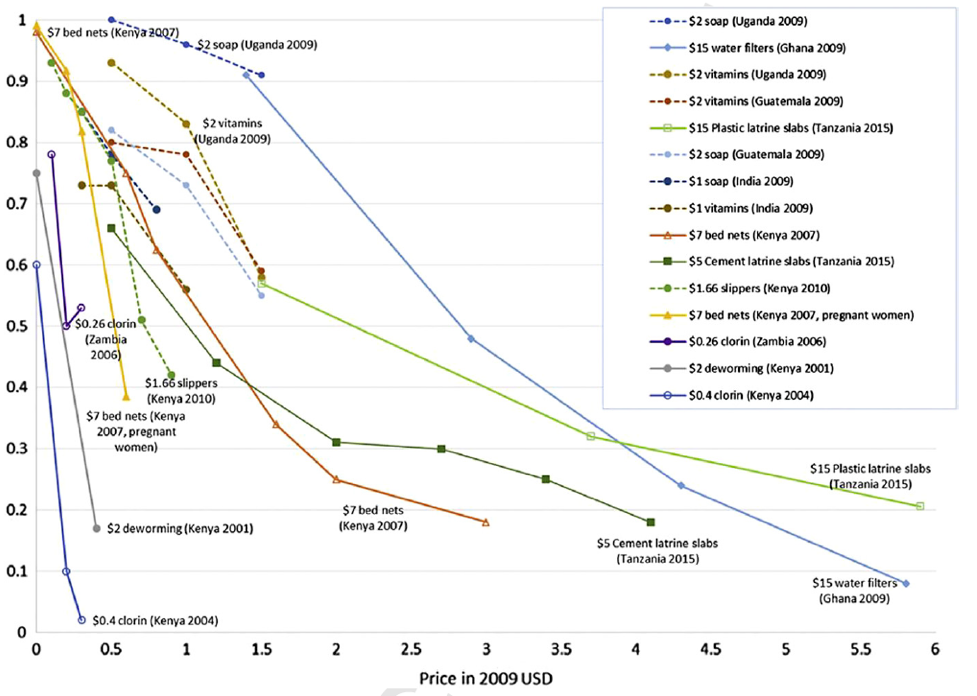
\includegraphics[width=85mm]{Picture2.png} \\
\caption{Share of individuals taking up the product as function of price (from \cite{dupas2017impacts})}
\end{center}
\end{figure}

\end{frame}

%%%%%%%%%%%%%%%%%%%%%%%%%%%%%%%%%%
\begin{frame}{High price sensitivity of demand for preventative health investments}
%%%%%%%%%%%%%%%%%%%%%%%%%%%%%%%%%%

\begin{wideitemize}

	\item High price-sensitivity even in cases of substantial long-run benefits:
	
    \begin{wideitemize}
    
        \item Deworming medication \citep{miguel2007worms}; mosquito nets \citep{cohen2010free}; water treatment \citep{ashraf2010can}.
    
        \item Example: estimated private financial benefit of deworming is \$142 \citep{baird2016worms}, yet \$0.30 per child cost-sharing fee decreased take up 80 percent \citep{miguel2007worms}.
        
    \end{wideitemize}

    \item High sensitivity also for monetary and non-monetary incentives: 
    
    \begin{itemize}
        
        \item Large impacts of small (and time-limited) incentives (lentils) for vaccination \citep{banerjee2010improving} or collecting HIV tests \citep{thornton2008demand}
        
        \item Prima facie evidence against liquidity constraints (though not conclusive)
        
    \end{itemize}
        
	\item If individuals are given more time to purchase, then lower price sensitivity, but demand still fairly sensitive to price \citep{dupas2009malariaprevent}.

	

\end{wideitemize}

\end{frame}

%%%%%%%%%%%%%%%%%%%%%%%%%%%%%%%%%%
\begin{frame}{Significant expenditures on acute conditions}
%%%%%%%%%%%%%%%%%%%%%%%%%%%%%%%%%%

\begin{wideitemize}

	\item Arguably excessive treatment for some acute conditions
	
	\item Lower price sensitivity for acute care \citep{Cohen2015}
	
	\item Suggests liquidity constraints cannot fully explain low demand for preventative health

\end{wideitemize}

\end{frame}


%%%%%%%%%%%%%%%%%%%%%%%%%%%%%%%%%%
\begin{frame}{Knife-edge balance between benefits and costs?}
%%%%%%%%%%%%%%%%%%%%%%%%%%%%%%%%%%

\begin{columns}[T] 

\begin{column}{.43\textwidth}
  
\begin{wideitemize}

	\item One possible explanation: some people are (close to) indifferent between investing and not investing.
	
	\item Small changes in prices or incentives can alter behavior.
	
	\item Unlikely explanation given that it requires that many people in different settings happen to be (close to) exactly indifferent.

\end{wideitemize}

\end{column}

\begin{column}{.53\textwidth}

\bigskip

\begin{figure}
    \centering
    \resizebox{\textwidth}{!}{
    
\includegraphics{Picture3.png} }
    \caption{Source: \cite{kremer2011improving,baird2016worms}}
    \label{fig:my_label}
\end{figure}

\end{column}

\end{columns}

\note{
    \begin{itemize}
        \item \textit{Knife-edge interpretation.} One story might be that people who do not take up preventive health goods perceive large benefits from preventive health investments, but they perceive even higher costs, and hence make a rational decision not to take up the preventive health measures.

        \item De-worming; Water treatment; Mosquito nets; HIV results

        \item The paper by Bryan et al (2014 ECMA) showing that a \$8 one-time subsidy can get people to migrate more to cities and earn 30\% more is another example of a small subsidy making a too-large difference to behaviors. 
    \end{itemize}
}

\end{frame}

%%%%%%%%%%%%%%%%%%%%%%%%%%%%%%%%%%
\begin{frame}{Can present bias explain under-investment in health?}
%%%%%%%%%%%%%%%%%%%%%%%%%%%%%%%%%%

\begin{wideitemize}

	\item Two ways present bias may generate this under-investment:

	\begin{wideitemize}

    \smallskip

		\item[(1)] Procrastination 

		\item[(2)] Liquidity constraints due to present bias

	\end{wideitemize}

\end{wideitemize}

\end{frame}

%%%%%%%%%%%%%%%%%%%%%%%%%%%%%%%%%%
\begin{frame}{Present bias and procrastination}
%%%%%%%%%%%%%%%%%%%%%%%%%%%%%%%%%%

\begin{wideitemize}

	\item Driven by the immediate \textit{utility costs} of the investment: 
	
	\begin{itemize}

	\item Examples: hassle and psychic costs of going to doctor, walking to farther-away water source, using dilute chlorine solution, changing diet, learning painful news about health status, taking medication.
	
	\item Not financial costs unless severely liquidity constrained

	\end{itemize}

	\item Procrastination requires both present bias and some degree of naivete. 
	
	\begin{itemize}
	
		\item Prefer to do painful task tomorrow, mis-predict that they will do it tomorrow.

	\end{itemize}

	\item Consistent with: 
	
	\begin{itemize}

		\item[(i)] effect of time-limited incentives: e.g.\ \cite{banerjee2010improving}
		
		\item[(ii)] effect of reducing hassle costs: e.g.\ water dispensers \citep{Ahuja2010}

	\end{itemize}

	\item \textit{Note:} Would not procrastinate on acute condition, since benefits immediate

\end{wideitemize}

\end{frame}

%%%%%%%%%%%%%%%%%%%%%%%%%%%%%%%%%%
\begin{frame}{Present bias and liquidity constraints}
%%%%%%%%%%%%%%%%%%%%%%%%%%%%%%%%%%

\begin{wideitemize}

	\item Present bias can lead to liquidity constraints \citep{angeletos2001hyperbolic}
	
	\item Once liquidity-constrained:

	\begin{itemize}
	
		\item High-return preventive investments may be left unexploited.
		
		\item Monetary expenditures might now translate into (almost) immediate utility costs, since need to cut back on other consumption in order to, e.g.\ pay for doctor visit.

	\end{itemize}
	
	\item Consistent with:

	\begin{itemize}

		\item Evidence on effects of increased liquidity \citep{dupas2013savings}
		
		\item High impact of small discounts to fertilizer around time of harvest \citep{duflo2011nudging}
		
	\end{itemize}

\end{wideitemize}

\end{frame}

%%%%%%%%%%%%%%%%%%%%%%%%%%%%%%%%%%
\begin{frame}{Methodological aside: Measuring demand with liquidity constraints}
%%%%%%%%%%%%%%%%%%%%%%%%%%%%%%%%%%

\begin{wideitemize}

	\item If people are liquidity constrained, surprising someone and offering to sell a good will not measure long-run demand.

	\item Endow people with money first?

	\begin{itemize}
	
		\item But how much money unclear in buffer stock world
		\item Can induce experimenter demand effects.

	\end{itemize}

	\item Give people time to buy the good \citep{dupas2009malariaprevent}
	
	\begin{itemize}
	
		\item Offer coupons, to reduce demand effects
		\item WTP underestimates welfare if present bias
	
	\end{itemize}

	\item Allow them to pay using credit?

\end{wideitemize}

\note{
    \begin{itemize}
    
        \item If people are present biased, they are likely to have liquidity constraints, and one should take care when trying to measure demand and draw welfare conclusions
        
        \item If costs are upfront and not smoothed over the lifetime, demand for durables will be under-estimated
    \end{itemize}
}

\end{frame}

%%%%%%%%%%%%%%%%%%%%%%%%%%%%%%%%%%
\begin{frame}{Present bias and commitment contracts}
%%%%%%%%%%%%%%%%%%%%%%%%%%%%%%%%%%

\begin{wideitemize}

	\item Demand for commitment is ``smoking gun" evidence of present bias \citep{ashraf2006tying,gine2010put,kaur2015self,schilbach2015alcohol,casaburi2018demand}.
	
	\item But commitment contracts only work well with high degree of sophistication
	
	\begin{itemize}
	
		\item Naivete $\rightarrow$ low demand for commitment
		
		\item Partial naivete $\rightarrow$ systematic failure of commitment, with plausibly negative effects on welfare if people incur the costs without the intended benefit \citep{john2016commitment,bai2017self}.
		
	\end{itemize}
	
	\item Uncertainty also implies low demand for commitment \citep{laibson2015don,Amador2006}.
	
	\item More promising approach may be to reduce hassle costs, provide direct time-limited incentives, ease liquidity constraints


\end{wideitemize}

\note{
    \begin{itemize}
    
    \scriptsize
    
        \item \cite{ashraf2006tying} (Tying Odysseus to the Mast): 28\% takeup of a commitment savings device in the Philippines; women who exhibited more present bias in hypothetical time preference questions were more likely to take up the contract. This suggests some sophistication. The commitment offer increased savings by 81 percentage points.

        \item \cite{gine2010put}: 11\% takeup among smokers of a commitment device (CARES) that allowed smokers to deposit money for six months, after which they would take a urine test for nicotine and cotinine. Failing the test forfeited the money. ITT: 3 percentage point increase in passing this test.

        \item \cite{duflo2008high} Duflo, Kremer, and Robinson: Small, time-limited discounts help present biased farmers commit to using fertilizer in the future.

        \item \cite{schilbach2015alcohol}: More than a third of subjects preferred incentives for sobriety to unconditional payments, even when the unconditional payments were strictly higher than the maximum amount they could earn with the incentives.

        \item \cite{bai2017self}: Hypertension patients in rural India. Moderate take-up of commitment, where individuals will put money on the line. But poor follow-through. Offering commitment makes consumers worse off on average, consistent with partial naivete. 

    \end{itemize}
}

\end{frame}


%%%%%%%%%%%%%%%%%%%%%%%%%%%%%%%%%%
\begin{frame}{Present bias, sophistication, and deadlines}
%%%%%%%%%%%%%%%%%%%%%%%%%%%%%%%%%%

\begin{wideitemize}

	\item The effect of naivete versus sophistication about one's present bias will depend on the nature of the investment in question. 
	
	\item Distinguish between 2 cases of high-return health investments:

	\begin{enumerate}[(I)]
	
	\item Case I: Investments without deadlines 
	
	\begin{itemize}
	
		\item Naive $\rightarrow$ repeated decisions to procrastinate
		\item Sophisticated $\rightarrow$ may delay for a few time periods but will eventually make investment therefore no major welfare losses
		\citep{ODonoghue2001}.
		
	\end{itemize}

	\item Case II: One-shot investments with deadlines (but negligible monetary costs)

	\begin{itemize}
	
		\item Even fairly present-biased agents will make the investment since there is no way to procrastinate.

	\end{itemize}
	
	\end{enumerate}

    \item While present bias can help explain some of the patterns in Case I, other decisions (especially in Case II) cannot be explained by present bias alone.
    
    \begin{itemize}
    
        \item Need other (additional) reasons than present bias to explain low demand, e.g.\ biased beliefs

    \end{itemize}
    
	
\end{wideitemize}

\end{frame}

%%%%%%%%%%%%%%%%%%%%%%%%%%%%%%%%%%
\begin{frame}{Biased beliefs}
%%%%%%%%%%%%%%%%%%%%%%%%%%%%%%%%%%

\begin{wideitemize}

	\item Making good decisions regarding health requires forming accurate beliefs about numerous variables. Difficult due to uncertainty and heterogeneity across individuals \citep{arrow1963uncertainty}.
	
	\item Inaccurate beliefs (e.g.\ misperceived returns to health investments) could help explain under-investment in health. Some evidence of inaccurate beliefs regarding health in developing societies (e.g.\ \cite{delavande2009subjective,godlonton2016responding}).

	\item Information interventions appear to have large impacts on health outcomes in some contexts and small to null in others \cite{dupas2011health,dupas2017impacts}. 
	
	\begin{itemize}
	    
	    \item Other behavioral biases might be at play in situations of low impacts of info.
	    
	    \item Motivated beliefs (e.g.\ deriving utility from belief that one is healthy) could matter as well.
	    
	    \item More work is required to understand the determinants of success in various contexts.
	    
	\end{itemize}
	
\end{wideitemize}

\end{frame}


%%%%%%%%%%%%%%%%%%%%%%%%%%%%%%%%%%
\begin{frame}{Incorrect causal theories or mental models}
%%%%%%%%%%%%%%%%%%%%%%%%%%%%%%%%%%

\begin{wideitemize}

	\item Individuals may interpret what they observe through the wrong causal model or theory \citep{schwartzstein2014selective,gagnon2017channeled}.
	
	\item Incorrect mental models that may be important for health outcomes in developing societies include superstitious beliefs or beliefs in magical theories of sickness and health which include witchcraft.
	
	\item \cite{ashraf2017traditional} illustrate this issue in the case of maternal risk in Zambia and a wide-spread belief about martial infidelity and complications during childbirth

	\item Parents across the world confidently hold wrong beliefs about need to re-hydrate  children in response to diarrhea. \cite{datta2014behavioral}: 30 to 50 percent of women in their sample (in India) recommended \textit{decreasing} fluid intake of infants to treat diarrhea


\end{wideitemize}

\end{frame}

%%%%%%%%%%%%%%%%%%%%%%%%%%%%%%%%%%
\begin{frame}{Evidence against importance of some ideas from psychology in the field}
%%%%%%%%%%%%%%%%%%%%%%%%%%%%%%%%%%

\begin{wideitemize}

	\item Little evidence for real-world development importance of some psychological effects frequently invoked by practitioners to justify policy:
	
	\bigskip
	
	\begin{wideitemize}

	\item \textbf{Sunk-cost fallacy:} No evidence that higher prices cause greater product use \cite{ashraf2010can,cohen2010free}. 
	\item \textbf{Crowd-out of intrinsic motivation:} Little evidence that extrinsic incentives crowd out intrinsic motivations in real world development contexts or that paying more leads to substantially less-motivated workers \citep{dal2013strengthening,ashraf2014no,ashraf2018losing}.
	
	\end{wideitemize}

\end{wideitemize}

\note{
    \begin{itemize}
        \item \cite{ashraf2014no}: Show this result among hairdressers in Zambia tasked with selling female condoms. Those who showed more concern about HIV/AIDS (measured through donations to a charity using a dictator game) responded more strongly to the incentives to sell condoms.

        \item \citet{ashraf2018losing}: Varied the salience of career incentives in job postings for community health workers in Zambia. This attracted more productive workers and increased output, suggesting that salient extrinsic incentives do not crowd out intrinsically-motivated agents.

        \item Dangers of setting policy based on behavioral claims without evidence.

    \end{itemize}
}

\end{frame}


%%%%%%%%%%%%%%%%%%%%%%%%%%%%%%%%%%
\section{4 Savings}
%%%%%%%%%%%%%%%%%%%%%%%%%%%%%%%%%%

%%%%%%%%%%%%%%%%%%%%%%%%%%%%%%%%%%
\begin{frame}{Topics covered}
%%%%%%%%%%%%%%%%%%%%%%%%%%%%%%%%%%

\small 

\begin{enumerate}[(1)]

	\item[(1)] Introduction 
	
	\item[(2)] {High rates of return without rapid growth (Euler equation puzzle)}

	\item[(3)] {Health}
	
	\item[(4)] \textbf{Savings}
		
	\item[(5)] Risk and insurance

	\item[(6)] Technology adoption
	
	\item[(7)] Labor

	\item[(8)] Firms
	
	\item[(9)] Social preferences, culture, and development
	
	\item[(10)] The psychology of poverty

\end{enumerate}

\end{frame}



%%%%%%%%%%%%%%%%%%%%%%%%%%%%%%%%%%
\begin{frame}{``Standard" barriers to saving}
%%%%%%%%%%%%%%%%%%%%%%%%%%%%%%%%%%

\begin{wideitemize}

	\item Savings are necessary to self-insure against risks and to finance lumpy investments 

	\item ``Standard" barriers to savings include: 
	
	\begin{itemize}
	
		\item Lack of access to formal savings products

		\item Prohibitive costs of opening a banking account etc.

	\end{itemize}
	
	\item \cite{dupas2018banking} find small effects of providing bank accounts to poor individuals, suggesting other (potentially behavioral) constraints may play a role in reducing savings


\end{wideitemize}

\end{frame}

%%%%%%%%%%%%%%%%%%%%%%%%%%%%%%%%%%
\begin{frame}{Commitment savings devices}
%%%%%%%%%%%%%%%%%%%%%%%%%%%%%%%%%%

\begin{wideitemize}

	\item A key prediction of present bias: households accumulate few liquid savings over time, while building up substantial illiquid wealth. Consistent with savings patters across the world \citep{angeletos2001hyperbolic,Banerjee2007,morduch2009portfolios}

	\item \cite{ashraf2006tying}: evidence for demand for commitment devices in the domain of savings which evidences present-bias (as discussed in Section 3.2).

	\item A key open question surrounding the usefulness of commitment devices is the optimal trade-off between commitment and flexibility. Too stringent commitment reduces take-up and too flexible commitment does not overcome self-control problems.

	\item \cite{dupas2013savings} find that a softer savings device increases spending on preventative care relative to a control group and a more stringent alternative.


\end{wideitemize}

\end{frame}

%%%%%%%%%%%%%%%%%%%%%%%%%%%%%%%%%%
\begin{frame}{Designing financial products for behavioral agents: Default effects}
%%%%%%%%%%%%%%%%%%%%%%%%%%%%%%%%%%

\begin{wideitemize}

	\item Setting default choices is a cheap but often highly powerful tool in changing behavior. 
	
	\item For instance, setting the default to automatic enrollment as opposed to non-enrollment has substantial impacts on individuals' retirement choices, particularly for lower-income individuals \citep{chetty2015behavioral, chetty2014active,madrian2001power}

	\item \cite{blumenstock2018defaults}: setting opt-in defaults increase the savings of Afghanistan workers. Additionally, they argue the underlying mechanism involves present bias as well as the hassle costs of thinking through different options.


\end{wideitemize}

\end{frame}

%%%%%%%%%%%%%%%%%%%%%%%%%%%%%%%%%%
\begin{frame}{Designing financial products for behavioral agents: Attention}
%%%%%%%%%%%%%%%%%%%%%%%%%%%%%%%%%%

\begin{wideitemize}

	\item Inattention can distort individuals' decision making in spheres ranging from savings to medical adherence and as such can have large costs.

	\item \cite{karlan2016getting} study the impact of reminders on savings and consumption choices and find that reminders increase the salience of savings goals.
    
    
    \item Many reminder interventions in health (e.g.\ \cite{PopEleches2011})
    
    %(Pop-Eleches et al., 2011; Raifman, et al., 2014; Lester et al., 2010).

	\item Potential negative externalities if attention is a limited resource. Need more evidence on whether reminders remain effective in the long term


\end{wideitemize}

\note{
    \begin{itemize}
        
        \item Pop-Eleches et al. and Lester et al. show that SMS reminders can increase adherence to antiretroviral therapy. 
        
        \item Raifman, et al., show that text message reminders can increase adherence to antimalarial treatment.

        \item Reminders: cognitive bandwidth literature (\cite{mullainathan2013scarcity}; \cite{schilbach2016psychological}) suggests that there may be negative externalities to text message reminders. May be useful to ask people whether they want reminders to avoid overload.
    \end{itemize}
}

\end{frame}

%%%%%%%%%%%%%%%%%%%%%%%%%%%%%%%%%%
\section{5 Risk and insurance}
%%%%%%%%%%%%%%%%%%%%%%%%%%%%%%%%%%

%%%%%%%%%%%%%%%%%%%%%%%%%%%%%%%%%%
\begin{frame}{Topics covered}
%%%%%%%%%%%%%%%%%%%%%%%%%%%%%%%%%%

\small 

\begin{enumerate}[(1)]

	\item[(1)] Introduction 
	
	\item[(2)] {High rates of return without rapid growth (Euler equation puzzle)}

	\item[(3)] {Health}
	
	\item[(4)] {Savings}
		
	\item[(5)] \textbf{Risk and insurance}

	\item[(6)] Technology adoption
	
	\item[(7)] Labor

	\item[(8)] Firms
	
	\item[(9)] Social preferences, culture, and development
	
	\item[(10)] The psychology of poverty

\end{enumerate}

\end{frame}



%%%%%%%%%%%%%%%%%%%%%%%%%%%%%%%%%%
\begin{frame}{Risk sharing}
%%%%%%%%%%%%%%%%%%%%%%%%%%%%%%%%%%

\begin{wideitemize}

	\item Major topic in development economics

	\begin{itemize}

		\item Large literature on informal risk sharing 

		\item Literature on how risk considerations affect input choices, migration, marriage, etc.

	\end{itemize}

	\item Warning: Aversion to small positive expected value gambles impossible to explain with expected utility theory \citep{rabin2000diminishing}


\end{wideitemize}

\end{frame}

%%%%%%%%%%%%%%%%%%%%%%%%%%%%%%%%%%
\begin{frame}{Low take-up of insurance}
%%%%%%%%%%%%%%%%%%%%%%%%%%%%%%%%%%

\begin{wideitemize}

	\item Many people in developing countries exposed to very risky income streams (e.g.\ farming)

	\item Yet low take up of actuarially fair weather insurance \citep{cole2013barriers}.

	\begin{itemize}

		\item Basis risk? \citep{clarke2011theory, mobarak2012selling,gine2008patterns} 
	
	\end{itemize}

	\item Low take-up of health insurance \citep{thornton2010}
	
	\begin{itemize}
	
		\item Administrative issues?

	\end{itemize}

\end{wideitemize}

\note{
    \begin{itemize}
        \item Little social insurance provided by the government
        
        \item Under most plausible utility functions, sharply diminishing marginal utility of income at very low consumption levels, so particularly strong need for insurance.
        
        \item Thornton et al. (2010): Nicaragua - voluntary health insurance scheme made available to informal workers through MFIs. Initial take up only 20\%. Less than 10\% of initial vendors still enrolled after one year.
    \end{itemize}
}


\end{frame}

%%%%%%%%%%%%%%%%%%%%%%%%%%%%%%%%%%
\begin{frame}{Potential explanations for low demand: Non-standard preferences}
%%%%%%%%%%%%%%%%%%%%%%%%%%%%%%%%%%

\begin{wideitemize}

	\item \cite{casaburi2018}: insurance meant to shift resources across states, yet most actual insurance contracts involve transferring resources over time % (not just across states).
	
	\begin{itemize}
	
		\item Eliminating the intertemporal component increases insurance take-up dramatically.
		
		\item Important role for liquidity constraints, present bias

	\end{itemize}
	
	\item Could loss aversion/prospect theory play a role?

	\begin{itemize}

        \item Reference-dependent preferences increase risk aversion over moderate stakes and may lead thus cause \textit{over-}insurance  \citep{sydnor2010over}.

		\item But premia might be seen as losses, thus curbing insurance demand \citep{eckles2011prospect}.
		
		\item Diminishing sensitivity away from reference point could lead to risk-seeking behavior in loss domain. 

	\end{itemize}

\end{wideitemize}

\note{
    \begin{itemize}
        \item \cite{casaburi2018}: Take-up of insurance where the premium is deducted at harvest time is 72\%, compared to 5\% for the standard contract with upfront payment of the premium. They argue that this is present bias for two reasons: (1) when people were given cash to cover the premium, finding that this did not substantially increase take up of the up front contract (suggesting that there's more to their result than just liquidity constraints), and (2) take-up of insurance where the premium delayed by a short amount of time (one month) was also high (21 percentage point above the standard contract). This effect size cannot be rationalized by standard exponential discounting, suggesting present bias.

        \item Loss aversion:
        reference points are important in determining the relationship between loss aversion and insurance demand:
        \begin{itemize}
            \item If a prospect theory actor uses initial wealth as his reference point, may consider the premium payment to be a loss, and  demand less insurance than a non-prospect-theory agent
            \item If instead uses initial wealth minus the premium as his reference point, will demand a higher level of insurance than a non-prospect-theory individual
        \end{itemize} 
    \end{itemize}
}

\end{frame}


%%%%%%%%%%%%%%%%%%%%%%%%%%%%%%%%%%
\begin{frame}{Potential explanations for low insurance demand: non-standard beliefs}
%%%%%%%%%%%%%%%%%%%%%%%%%%%%%%%%%%

	\begin{wideitemize}
	
		\item \textbf{Projection bias:} In good states of the world, agents may underestimate their marginal utility in bad states of the world \citep{loewenstein2003projection}.

		\item \textbf{Recency effects:} Agents might place disproportionate weight on events from the recent past \citep{hogarth1992order,fuster2010natural,chang2016something,karlan2014agricultural}.

		\item \textbf{Motivated reasoning:} If individuals directly derive utility from beliefs about their future well-being, they may seek to maintain biased beliefs about their current health or the likely future state of the world.

        \item \textbf{Beliefs in higher powers:} Individuals' beliefs might deviate in more dramatic ways from standard probability assessments. Beliefs in higher powers might suppress insurance demand \citep{auriol2018god}.

	\end{wideitemize}

\end{frame}


%%%%%%%%%%%%%%%%%%%%%%%%%%%%%%%%%%
\section{6 Technology}
%%%%%%%%%%%%%%%%%%%%%%%%%%%%%%%%%%

%%%%%%%%%%%%%%%%%%%%%%%%%%%%%%%%%%
\begin{frame}{Topics covered}
%%%%%%%%%%%%%%%%%%%%%%%%%%%%%%%%%%

\small 

\begin{enumerate}[(1)]

	\item[(1)] Introduction 
	
	\item[(2)] {High rates of return without rapid growth (Euler equation puzzle)}

	\item[(3)] {Health}
	
	\item[(4)] {Savings}
		
	\item[(5)] {Risk and insurance}

	\item[(6)] \textbf{Technology adoption}
	
	\item[(7)] Labor

	\item[(8)] Firms
	
	\item[(9)] Social preferences, culture, and development
	
	\item[(10)] The psychology of poverty

\end{enumerate}

\end{frame}


%%%%%%%%%%%%%%%%%%%%%%%%%%%%%%%%%%
\begin{frame}{Technology adoption}
%%%%%%%%%%%%%%%%%%%%%%%%%%%%%%%%%%

\begin{wideitemize}

	\item Various examples with apparently non-optimal technology choice:

	\begin{itemize}
	
		\item Pineapple farming in Ghana, HYV seeds, seaweed pod size, fertilizer, contraceptives, soccer ball manufacturing techniques, layout of equipment in textile factories

	\end{itemize}

	\item Do external analysts correctly understand payoffs?

	\item Do decision makers have adequate information?

	
\end{wideitemize}

\end{frame}




%%%%%%%%%%%%%%%%%%%%%%%%%%%%%%%%%%
\begin{frame}{Technology adoption: attention and complexity}
%%%%%%%%%%%%%%%%%%%%%%%%%%%%%%%%%%

\begin{wideitemize}

	\item Inattention and wrong mental models \citep{hanna2014learning} 

	\begin{itemize}

		\item Production function is complex and attention is costly. 
		
		\item Individuals will pay attention to the dimensions they think are important.

		\item If start off thinking something is not important (wrong mental model), will not pay attention and will never learn, even with data that would otherwise lead to revision of beliefs.

	\end{itemize}

	\item Complexity of information

	\begin{itemize}
	
		\item Provision of simplified information about seaweed pod size \citep{hanna2014learning}, water safety \citep{bennear2013impact} or business practices \citep{drexler2014keeping} may be more effective than providing full information.

        \item Downsides of presenting simplified information: heterogeneity in population; external analysts might misunderstand decision problem

	\end{itemize}
	
\end{wideitemize}

\note{
    \begin{itemize}
        \item \cite{hanna2014learning}:  Experienced seaweed farmers in Indonesia do not attend to pod size when planting seaweed. In the baseline, they cannot report the size they use or the optimal size. This is even though their existing plots provide plenty of unintentional experiments: variation in initial pod size which affects final size and profits. The theory is that they do not think pod size is important, so they do not pay attention to it, so they never learn even though in principle have all the data they need.

        \item When they are presented with the data in full detail, they still do not change their behaviors. But when they are presented with simple summary results of the trial on their plot, they do change behavior. 
        \end{itemize}
}

\end{frame}

%%%%%%%%%%%%%%%%%%%%%%%%%%%%%%%%%%
\begin{frame}{Technology adoption: present bias and loss aversion}
%%%%%%%%%%%%%%%%%%%%%%%%%%%%%%%%%%

\begin{wideitemize}

	\item Present bias \citep{duflo2011nudging}
	
	\begin{itemize}
	
		\item If adoption requires costly experimentation, individuals might procrastinate since benefits are often much delayed.
		
		\item Could benefit from simplification (if learning is costly). 

		\item Is there demand for commitment for technology adoption (training)? 
		
		\item Time-limited discounts around harvest highly effective at increasing take-up of fertilizer
		
	\end{itemize}

	\item Loss aversion

	\begin{itemize}

		\item Conjecture: relevant reference point when trying something new is the status quo. Possibility of losses with respect to the status quo will trigger loss aversion
		
		\item Possibility of insurance or informal risk-sharing to improve outcomes? 

	\end{itemize}
	
\end{wideitemize}

\end{frame}

%%%%%%%%%%%%%%%%%%%%%%%%%%%%%%%%%%
\begin{frame}{Behavioral social learning}
%%%%%%%%%%%%%%%%%%%%%%%%%%%%%%%%%%

\begin{wideitemize}

	\item Rational social learning will often lead society to right long-run choice if some can get past initial experimentation costs

	\item \cite{banerjee1992simple} herd behavior: model converges on optimal technology if: 

	\begin{itemize}
	
		\item observe output

		\item observe size of investment

		\item smooth loss function makes choices reveal signals 

	\end{itemize}

	\item Why might individuals not converge on optimal technology? We distinguish:
	
	\begin{enumerate}[(1)] 
	
		\item Barriers to sharing or seeking information
		
		\item Barriers to correctly interpreting information

	\end{enumerate}
	
\end{wideitemize}

\note{
    \begin{itemize}
        \item \cite{foster1996technical} suggests rapidly adopt green revolution technology but this was a very beneficial technology

        \item \cite{banerjee1992simple}: Herding would not go through if each person's choice was a sufficient statistic for their information.

    \end{itemize}

}

\end{frame}

%%%%%%%%%%%%%%%%%%%%%%%%%%%%%%%%%%
\begin{frame}{Barriers to sharing and seeking information: Social-image concerns}
%%%%%%%%%%%%%%%%%%%%%%%%%%%%%%%%%%

\begin{wideitemize}

	\item The degree of communication between people is endogenous. Providing and soliciting information is a decision.

	\item People may be hesitant to ask for or provide information when doing so signals effort or ability (\cite{Chandrasekhar2018,banerjee2018}; 
	
	\begin{itemize}
	
		\item Implies seeding info more broadly can reduce learning
	
	\end{itemize}
	
	\item People may not be willing to provide information to others for free if they paid for it or put in effort to get it.

	
\end{wideitemize}

\end{frame}

%%%%%%%%%%%%%%%%%%%%%%%%%%%%%%%%%%
\begin{frame}{Barriers to interpreting information: Redundancy neglect}
%%%%%%%%%%%%%%%%%%%%%%%%%%%%%%%%%%

\begin{wideitemize}

    \item \cite{benjamin2018errors}: review of biases in learning and errors in probabilistic reasoning.

    \begin{itemize}
    
    	\item Plenty of lab evidence but limited field evidence, e.g.\ on how non-Bayesian social learning influences technology adoption. Lots of opportunities!
    
    \end{itemize}

	\item Theoretical work: imitating common sources without accounting for redundancy in the signals received can create confident and incorrect beliefs \citep{eyster2014extensive}.

	\begin{itemize}

		\item People may overweight the beliefs and actions of others.

	\end{itemize}

	\item Empirical evidence of naive, non-Bayesian updating
	
	\begin{itemize}

		\item People neglect the correlation of information structures resulting in double-counting of signals \citep{enke2013correlation}.

		\item Rather than using Bayes' Rule to evaluate the state of the world, people use a weighted average of neighbors' actions or opinions \citep{Chandrasekhar2015}
		
	\end{itemize}

	\item This may create information traps, making it hard to encourage adoption of technologies that go against conventional wisdom. 

	
\end{wideitemize}

\end{frame}


%%%%%%%%%%%%%%%%%%%%%%%%%%%%%%%%%%
\section{7 Labor}
%%%%%%%%%%%%%%%%%%%%%%%%%%%%%%%%%%

%%%%%%%%%%%%%%%%%%%%%%%%%%%%%%%%%%
\begin{frame}{Topics covered}
%%%%%%%%%%%%%%%%%%%%%%%%%%%%%%%%%%

\small 

\begin{enumerate}[(1)]

	\item[(1)] Introduction 
	
	\item[(2)] {High rates of return without rapid growth (Euler equation puzzle)}

	\item[(3)] {Health}
	
	\item[(4)] {Savings}
		
	\item[(5)] {Risk and insurance}

	\item[(6)] {Technology adoption}
	
	\item[(7)] \textbf{Labor}

	\item[(8)] Firms
	
	\item[(9)] Social preferences, culture, and development
	
	\item[(10)] The psychology of poverty

\end{enumerate}

\end{frame}



%%%%%%%%%%%%%%%%%%%%%%%%%%%%%%%%%%
\begin{frame}{Distinct features of labor markets in developing economies}
%%%%%%%%%%%%%%%%%%%%%%%%%%%%%%%%%%

\begin{wideitemize}

	\item Labor markets in developing economies are different to labor markets in rich countries in three key ways that make behavioral biases potentially more important:

	\begin{wideitemize}
	
	\bigskip
	
		\item High levels of informality
		
		\item High levels of casual labor

		\item High degree of self employment

	\end{wideitemize}
	
\end{wideitemize}

\end{frame}

%%%%%%%%%%%%%%%%%%%%%%%%%%%%%%%%%%
\begin{frame}{Distinct features of labor markets in developing economies (cont'd)}
%%%%%%%%%%%%%%%%%%%%%%%%%%%%%%%%%%

\begin{wideitemize}

	\item Preference for work-hour flexibility might differ between developed and developing economies due to social expectations and strategic complementarities. 

	\item View consistent with observed wage premium for formal sector jobs as well as high absence rates of employees in private sector jobs in developing countries \citep{kremer2005teacher}

	\item \cite{blattman2018impacts} randomly assign industrial jobs in Ethiopia, finding that workers quickly quit and move to different sectors.

	
\end{wideitemize}

\note{
    \begin{itemize}
        \item \cite{blattman2018impacts}: Trade-off: volatile and risky self employment vs. poor working conditions of industrial jobs. People who were offered industrial jobs accepted but left quickly, using them as an income source while looking for other work. Workers seemed to understand the risks, but found the industrial jobs unpleasant. When the barriers to entry were alleviated, people preferred entrepreneurial work to industrial work.

        \item \cite{mas2017valuing} show that most workers in the U.S. do NOT value flexible scheduling, and that most people want to work 40 hours per week. People are particularly averse to jobs with employer discretion in scheduling, and are willing to take a (on average) 20\% pay cut to avoid this arrangement.

    \end{itemize}

}

\end{frame}

%%%%%%%%%%%%%%%%%%%%%%%%%%%%%%%%%%
\begin{frame}{Labor supply and worker productivity}
%%%%%%%%%%%%%%%%%%%%%%%%%%%%%%%%%%

\begin{wideitemize}

	\item One implication of informal work and self-employment is that workers might be more influenced by behavioral biases -- as seen, for instance, in the high rates of inebriation during the work-day documented in \cite{schilbach2015alcohol}.

	\item Self-control problems in a workplace setting are different to other domains in that, in addition to reducing the worker's welfare, they can reduce firm profits.

	
\end{wideitemize}

\end{frame}

%%%%%%%%%%%%%%%%%%%%%%%%%%%%%%%%%%
\begin{frame}{Factory discipline as commitment device}
%%%%%%%%%%%%%%%%%%%%%%%%%%%%%%%%%%

\begin{wideitemize}

	\item \cite{clark1994factory} argues workers want factory discipline as a commitment device.

	\begin{itemize}

		\item Much rosier view 

	\end{itemize}

	\item \cite{kaur2015self}

	\begin{itemize}

		\item About a third of data-entry workers choose dominated commitment contract over piece rate contract
		
		\item Offering dominated contract increases output.
		
		\item Substantial heterogeneity; some evidence of learning

		\item With asymmetric information, firms may screen out undesirable workers with factory discipline or steep incentives, reducing overall welfare

		\item Justification for legislation limiting hours, etc.?

	\end{itemize}
	
\end{wideitemize}

\end{frame}

%%%%%%%%%%%%%%%%%%%%%%%%%%%%%%%%%%
\begin{frame}{Wage rigidities}
%%%%%%%%%%%%%%%%%%%%%%%%%%%%%%%%%%

\begin{wideitemize}

	\item The share of the population employed in agriculture is much higher in poor countries than in rich countries. And most farms employ outside workers for short spells using informal contracts \cite{kaur2014nominal}.

	\item Agricultural labour markets have many features that ostensibly should make them efficient: many small buyers and sellers of labor, no formal unions and little to no enforcement of minimum wages

	\item Despite this, even in these decentralized informal markets, nominal wage rigidities and limited dispersion of wages across workers persist. \citep{kaur2014nominal,breza2017morale,brezascabs}.
	
	
\end{wideitemize}

\end{frame}

%%%%%%%%%%%%%%%%%%%%%%%%%%%%%%%%%%
\begin{frame}{Why do wage rigidities persist?}
%%%%%%%%%%%%%%%%%%%%%%%%%%%%%%%%%%

\begin{wideitemize}

	\item Wage rigidities seem persistent even in the absence of enforced minimum wages or formal institutions like unions.

	\item These rigidities appear to be enforced via \textbf{social sanctions}:

	\begin{itemize}

		\item \cite{brezascabs}: nominal wage rigidities persist in part due to workers turning down public offers of jobs with wages below the prevailing market wage which workers accept when those offers are made in private.

		\item \cite{breza2017morale}: when coworker productivity is difficult to observe, then introducing pay inequality reduces worker output.
		
	\end{itemize}

	
\end{wideitemize}

\end{frame}

%%%%%%%%%%%%%%%%%%%%%%%%%%%%%%%%%%
\begin{frame}{Wages and incentives to do good}
%%%%%%%%%%%%%%%%%%%%%%%%%%%%%%%%%%

\begin{wideitemize}

	\item \textbf{Incentives in public and non-profit sectors:}
	
	\begin{itemize}

		\item Some evidence of positive effects of financial incentives on public/non-profit sector worker productivity \citep{duflo2012incentives,muralidharan2011teacher}

		\item But providing incentives to multi-tasking agents is difficult \citep{holmstrom1991multitask}.
		
		\item Additionally, financial incentive programs tend to be politically unpopular and therefore are rarely scaled by governments \citep{finan2017personnel}

	\end{itemize}

	\item \textbf{Crowd-out intrinsic motivation:}
	
	\begin{itemize}

		\item Lab evidence suggests extrinsic rewards can reduce intrinsic motivation \citep{deci1971effects,benabou2003intrinsic}

		\item But very limited field evidence of substantial crowding out \citep{lacetera2013economic}

	\end{itemize}
	
\end{wideitemize}

\end{frame}

%%%%%%%%%%%%%%%%%%%%%%%%%%%%%%%%%%
\begin{frame}{Selection of workers}
%%%%%%%%%%%%%%%%%%%%%%%%%%%%%%%%%%

\begin{wideitemize}

	\item Does offering higher wages, which might attract more talent, negatively select on the pro-social motivation of workers?

	\item Majority of evidence suggests no negative selection.
	\cite{dal2013strengthening} in Mexico and \cite{ashraf2018losing}, in Zambia. 
	
	\item Evidence consistent with underlying correction of cognitive ability and pro-sociality \citep{falk2018global}.
	
	\item However, \cite{deserranno2017financial} finds that posting job notices with a higher implied pay attracts candidates who donate less money in dictator games, and who perceive lower social benefits to the job at the time of applying. 

	
\end{wideitemize}

\note{
    \begin{itemize}
        \item \cite{dal2013strengthening}
        work with the Mexican federal government to randomize wage offers across 167 municipalities to fill 350 positions. Applicants complete a battery of tests of ability, personality traits and pro-social motivations. The authors find that higher wage offers attract a higher-ability applicant pool in terms of fluid intelligence, better personality traits, and experience. Yet this increase in applicants did not come with a cost in terms of lower public-service motivation (measured using survey questions). \cite{ashraf2018losing} find similar results with a field experiment in Zambia, where they vary across locations whether job postings to recruit health workers emphasized either career prospects or instead the possibility of helping one's community. Emphasizing career prospects led to recruiting applicants with higher high-school grades, but no lower prosocial motivation.

    \end{itemize}

}

\end{frame}

%%%%%%%%%%%%%%%%%%%%%%%%%%%%%%%%%%
\begin{frame}{Female labor force participation (FLFP)}
%%%%%%%%%%%%%%%%%%%%%%%%%%%%%%%%%%

\begin{wideitemize}

	\item 52\% of women in poor countries participate in the labour force compared to 78\% of men \citep{duflo2012incentives}

	\item Standard explanations emphasize biological reasons which, it is typically argued, engender differences in the specialization of the sexes between wage work and domestic work.

	\item Leaves much of the variation in FLFP unexplained, even conditional on income per capita.

	\item Behavioral explanations include:

	\begin{itemize}
	
		\item Low self-efficacy \citep{mckelway2018women}
		
		\item Social norms suppressing FLFP \citep{bursztyn2018misperceived}

	\end{itemize}
		
\end{wideitemize}

\end{frame}


%%%%%%%%%%%%%%%%%%%%%%%%%%%%%%%%%%
\section{8 Firms}
%%%%%%%%%%%%%%%%%%%%%%%%%%%%%%%%%%

%%%%%%%%%%%%%%%%%%%%%%%%%%%%%%%%%%
\begin{frame}{Topics covered}
%%%%%%%%%%%%%%%%%%%%%%%%%%%%%%%%%%

\small 

\begin{enumerate}[(1)]

	\item[(1)] Introduction 
	
	\item[(2)] {High rates of return without rapid growth (Euler equation puzzle)}

	\item[(3)] {Health}
	
	\item[(4)] {Savings}
		
	\item[(5)] {Risk and insurance}

	\item[(6)] {Technology adoption}
	
	\item[(7)] {Labor}

	\item[(8)] \textbf{Firms}
	
	\item[(9)] Social preferences, culture, and development
	
	\item[(10)] The psychology of poverty

\end{enumerate}

\end{frame}


%%%%%%%%%%%%%%%%%%%%%%%%%%%%%%%%%%
\begin{frame}{Behavioral firms}
%%%%%%%%%%%%%%%%%%%%%%%%%%%%%%%%%%

\begin{wideitemize}

	\item Is it reasonable to assume firms (as opposed to individuals) make choices that maximize profits? Are there reasons to believe firms in developing economies are more behavioral?
	
	\begin{itemize}
	    
	    \item Here: broad definition of ``behavioral": deviations from profit maximizing behavior
	    
	\end{itemize}

	\item \cite{lucas1978size} span of control model and Chicago critique of behavioral economics:

	\begin{itemize}
	
		\item Behavioral firms will be weeded out of the market.
		
		\item Even if only 5\% of people don't have behavioral biases, they will become managers of firms.

	\end{itemize}
	
	\item Distortions in developing countries prevent efficient firms from growing and displacing less efficient ones.

	\item Self-employed individuals in developing countries are not just behavioral consumers, they are behavioral firms -- or at least behavioral managers. 

	
\end{wideitemize}

\end{frame}

%%%%%%%%%%%%%%%%%%%%%%%%%%%%%%%%%%
\begin{frame}{Reasons developing economy firms could be more behavioral}
%%%%%%%%%%%%%%%%%%%%%%%%%%%%%%%%%%

\begin{wideitemize}

	\item[(1)] Lower competitive pressures due to:

	\begin{wideitemize}
	
    \smallskip

		\item[(i)] Import restrictions

		\item[(ii)] Restriction of new entrants into markets based on regulation, financial constraints, and agency problems

	\end{wideitemize}

\end{wideitemize}

\end{frame}


%%%%%%%%%%%%%%%%%%%%%%%%%%%%%%%%%%
\begin{frame}{Reasons developing economy firms could be more behavioral (cont'd)}
%%%%%%%%%%%%%%%%%%%%%%%%%%%%%%%%%%

\begin{wideitemize}

	\item[(2)] Smaller firm sizes which limit the scope for within-firm competition that causes non-behavioral agents to rise to management:

    \smallskip

	\begin{wideitemize}

		\item[(i)] Smaller firm sizes as discussed in the previous chapter potentially due to:

		\begin{itemize}

			\item Taxation and regulation (e.g. labor regulation), predation

			\item Credit market issues (But profitable firms should grow over time?)

			\item Correlation between firm size and family structure (\cite{ilias2006families}; \cite{bertrand2008mixing})

            \item Difficulty of cooperation?
		
		\end{itemize}

		\item[(ii)] Implications
	
		
		\begin{itemize}
		
			\item Firms may only replace self employment when productivity advantage becomes large enough to outweigh these costs.

			\item Reduces ability of innovations to spread, incentives to innovate

			\item Reduces replacement of inefficient producers

		\end{itemize}	

	\end{wideitemize}

\end{wideitemize}

\note{
    \begin{itemize}
        \item \cite{ilias2006families}: Family firms are organizational ways of dealing with agency costs. Consistent with this, Ilias shows that there is a positive relationship between family size and firm size in the surgical instrument industry in Pakistan. Firm founders with more brothers (and therefore a larger pool of managers) end up with larger firms.

        \item \cite{bertrand2008mixing}: Study 93 large business families in Thailand. They find a positive relationship between family size and family involvement in the company. In particular when the founder is dead, the sons play a larger role in the company, and greater sons' involvement when the founder is dead is associated with lower firm-level performance (their interpretation: a ``race to the bottom" to tunnel out resources). 
    \end{itemize}


}

\end{frame}

%%%%%%%%%%%%%%%%%%%%%%%%%%%%%%%%%%
\begin{frame}{Reasons developing economy firms could be \textit{less} behavioral}
%%%%%%%%%%%%%%%%%%%%%%%%%%%%%%%%%%

\begin{wideitemize}

	\item Higher stakes for self-employed owners of small firms

    \begin{itemize}
        
        \item But: behavioral biases also important in high-stakes settings (e.g.\ 401k savings)
        
        \item Also: consumption closely linked to profits and revenue, so behavioral biases (e.g.\ present bias, loss aversion) might have more bite
        
    \end{itemize}

	\item Many seemingly-identical firms (e.g.\ small shops selling identical products) suggesting high levels of competition

	
\end{wideitemize}

\end{frame}


%%%%%%%%%%%%%%%%%%%%%%%%%%%%%%%%%%
\begin{frame}{Behavioral firms: low levels of trust}
%%%%%%%%%%%%%%%%%%%%%%%%%%%%%%%%%%

\begin{wideitemize}

	\item Once we start considering behavioral biases in firm decision-making, many unexplored and potentially important areas of research arise. 
	
	\item Example: Low levels of trust and missing firm growth:

	\begin{itemize}
	
		\item Firms in developing countries are small and standard explanations do not completely account for just how small these firms tend to be.
	
		\item Low levels of trust associated with smaller firm sizes \cite{cingano2012trust,algan2014trust}
		
		\item Non-Western countries are more likely to emphasize loyalty to one's group \citep{haidt2012righteous}, which might in turn limit cooperation with out-group members.

	\end{itemize}
	
\end{wideitemize}

\note{
    \begin{itemize}
        \item Standard explanations for small firms include taxation, regulation (e.g. labor regulation), and predation. While these factors may well play some role, many firms are even smaller than these thresholds (e.g. \cite{hsieh2014missing}), suggesting there may be additional reasons for firms to fail to grow.
    \end{itemize}

}

\end{frame}

%%%%%%%%%%%%%%%%%%%%%%%%%%%%%%%%%%
\begin{frame}{Behavioral firms: management practices}
%%%%%%%%%%%%%%%%%%%%%%%%%%%%%%%%%%

\begin{wideitemize}

	%\item Another related potential research horizon: management practices
	
	\item Improved management practices have been shown to increase firm profitability in developing country contexts \citep{bloom2013does,bruhn2018impact}.
		
	\item Why are such services not demanded and offered more?
		
	\item Firms that fail to adopt these profitable practices are not necessarily weeded out of the market. 

\end{wideitemize}

\note{
    \begin{itemize}
        \item \cite{bloom2013does} investigate firms' management practices by running a management field experiment with large, multi-plant textile firms in India. Firms in this study receive free consulting on management practices to a treatment group of firms and find that this intervention increases productivity by 17\% in the first year. Annual profitability increased by over \$300,000, and treatment firms grew faster and opened more production plants within three years.

        \item \cite{bruhn2018impact} examines the impact of access to one year of management consulting services on the outcomes of small and medium enterprises in Mexico. The authors randomly assigned enterprises that applied to receive subsidized consulting services to either receive the subsidized services or not. The authors find that the consulting intervention increased owners' ``entrepreneurial spirit" (an index that measures entrepreneurial confidence and goal setting) and had positive short-run impacts on productivity and profits.
    \end{itemize}

}

\end{frame}

%%%%%%%%%%%%%%%%%%%%%%%%%%%%%%%%%%
\begin{frame}{New research horizons associated with behavioral firms}
%%%%%%%%%%%%%%%%%%%%%%%%%%%%%%%%%%

\begin{wideitemize}

	\item Lots of unexplored areas waiting to be explored:

	\begin{wideitemize}

    \smallskip
    
		\item The nature of the objective function of small (family) businesses 

        \item Demand forecasting/estimating by firms

		\item Optimality of pricing or product choices amongst firms

		\item Inventory management

		\item Firm labor and capital-investment decisions

		\item Technology adoption

	\end{wideitemize}
	
\end{wideitemize}

\end{frame}

%%%%%%%%%%%%%%%%%%%%%%%%%%%%%%%%%%
\section{9 Social prefs}
%%%%%%%%%%%%%%%%%%%%%%%%%%%%%%%%%%

%%%%%%%%%%%%%%%%%%%%%%%%%%%%%%%%%%
\begin{frame}{Topics covered}
%%%%%%%%%%%%%%%%%%%%%%%%%%%%%%%%%%

\small 

\begin{enumerate}[(1)]

	\item[(1)] Introduction 
	
	\item[(2)] {High rates of return without rapid growth (Euler equation puzzle)}

	\item[(3)] {Health}
	
	\item[(4)] {Savings}
		
	\item[(5)] {Risk and insurance}

	\item[(6)] {Technology adoption}
	
	\item[(7)] {Labor}

	\item[(8)] Firms
	
	\item[(9)] \textbf{Social preferences, culture, and development}
	
	\item[(10)] The psychology of poverty

\end{enumerate}

\end{frame}


%%%%%%%%%%%%%%%%%%%%%%%%%%%%%%%%%%
\begin{frame}{Trust, cooperation, and development}
%%%%%%%%%%%%%%%%%%%%%%%%%%%%%%%%%%

\begin{wideitemize}

	\item Trust and cooperation important for economic and political outcomes 

	\begin{itemize}
	
		\item e.g.\ \cite{algan2014trust} review

	\end{itemize}

	\item Developing countries have lower levels of trust and positive reciprocity 

	\begin{itemize}
	
		\item \cite{falk2018global} using global survey 

	\end{itemize}
	
	\item Is this a cause or consequence of development?

	
\end{wideitemize}

\end{frame}

%%%%%%%%%%%%%%%%%%%%%%%%%%%%%%%%%%
\begin{frame}{Trust, cooperation, and development (cont'd)}
%%%%%%%%%%%%%%%%%%%%%%%%%%%%%%%%%%

\begin{wideitemize}

	\item Good reasons to think that variation in trust and reciprocity have deep historical roots
    
    \begin{wideitemize}

    \smallskip

	\item \cite{enke2008kinship}: historical tightness of kinship predicts modern-day in-group favoritism, willingness to cheat on and distrust outsiders, local rather than broader institutions. 

	\item \cite{nunn2011slave}: long-term consequences of slave trade

	\item \cite{henrich2010markets}: evolution of fairness and punishment facilitated trust and cooperation, allowing for large-scale societies 
	
	\begin{itemize}
	
		\item E.g., moralizing gods and cooperation with strangers?

		\item Market integration and fairness; community size and punishment

	\end{itemize}

    \end{wideitemize}


	\item But likely also in part a consequence of development, e.g.\ market exposure and well-functioning legal institutions might themselves increase trust.

	
\end{wideitemize}

\note{ 
    \begin{itemize}
        \item \cite{henrich2010markets} (with different coauthors) has argued that the emergence of large-scale societies required the ability to cooperate with strangers  in one-shot settings.
        
        \begin{itemize}
            \item He argues that this was facilitated by cultural evolution which favored pro-sociality, norm adherence and the willingness to punish norm violations. 
        
            \item The emergence of moralizing gods, for instance, was a cultural tool which helped people cooperate with strangers. The evidence is hard to evaluate, since they try to explain tens of facts rather than through any one clear test.
        \end{itemize} 
        
        \item \cite{henrich2010markets} show that market integration (measured as the percentage of purchased calories) positively co-varies with fairness while community size positively co-varies with punishment.

    \end{itemize}
}

\end{frame}

%%%%%%%%%%%%%%%%%%%%%%%%%%%%%%%%%%
\begin{frame}{Social image and norms}
%%%%%%%%%%%%%%%%%%%%%%%%%%%%%%%%%%

\begin{wideitemize}

	\item Frontier of behavioral research on (pro)social behavior is on social image

	\begin{itemize}
	
		\item Desire to conform to social norms
		
		\item And also to impress (in socially sanctioned ways)

		\item Visibility of actions can matter a great deal

	\end{itemize}

	\item Some recent applications

	\begin{itemize}
	
		\item \citet{platinum} on conspicuous consumption in Indonesia

		\item \cite{Chandrasekhar2018,Chandrasekhar2015,banerjee2018}
		on social learning

	\end{itemize}

	\item Much more work to be done in developing-country settings

	\begin{itemize}

		\item Including on how norms change, e.g.\ gender norms

	\end{itemize}
	
\end{wideitemize}

\note{
    \begin{itemize}
        \item \citet{platinum} show that middle class and wealthy people in Indonesia buy status goods -- in their case exclusive credit cards -- in large part to signal their high income to others, creating positional externalities through ``wasteful" expenditure. They also show that having higher self-esteem causally reduces demand for these types of goods. One interpretation is that having lower self esteem -- which is correlated with poverty -- makes people particularly eager to earn a high social image. 

    \end{itemize}
}

\end{frame}

%%%%%%%%%%%%%%%%%%%%%%%%%%%%%%%%%%
\begin{frame}{Shaping social preferences and norms}
%%%%%%%%%%%%%%%%%%%%%%%%%%%%%%%%%%

\begin{wideitemize}

	\item Important to understand policies which can improve inter-group behaviors

	\begin{itemize}

		\item \cite{rao2018familiarity} on integration in schools

		\item \cite{blouin2017erasing}
		on post-conflict Rwanda

        \item \cite{lowe2018unity} on different types of contact

        \item \cite{okunogbe2018does} on consequences of national service in Nigeria
	
		\item \cite{miguel2004tribe} on national identity in Tanzania
	
		\item Role of policy and culture \citep{miguel2005ethnic}

	\end{itemize}

	\item And policies which can influence certain social norms

	\begin{itemize}
	
		\item \cite{la2012soap}; \cite{jensen2009power}: TV effects on fertility, gender attitudes

		\item \cite{bursztyn2018misperceived} on female labor force participation in Saudi Arabia

	\end{itemize}
	
\end{wideitemize}

\note{ 
    \begin{itemize}
        \item \cite{rao2018familiarity}  shows how integration of rich and poor children in schools reduces discrimination and increases willingness to socialize, generosity and inequity-aversion. 

        \item \cite{blouin2017erasing} show that govt radio in Rwanda changes how people categorize others. It makes them less likely to categorize others using ethnicity -- measured by how likely they are to misattribute a fact about Person A to being about Persons B or C, depending on the ethnicity match between the individuals. They also show some evidence that trust between Hutus and Tutsis increases due to the radio channel. 

        \item \cite{la2012soap} show that telenovelas in Brazil reduced fertility for the exposed cohorts in the exposed regions. \cite{jensen2009power} show that cable TV changes stated gender attitudes. 

        \item \cite{bursztyn2018misperceived} are studying what whether male support for female labor force participation in Saudi Arabia can be changed by debiasing second-order beliefs. The idea is that men state in private that they do not mind their wives working, but believe that other men mind. Thus, they may try to keep their wives from working, fearing social disapproval. Once you inform them that ``80\% of men actually say they do not mind", one might be able to rapidly change the social norm. 

    \end{itemize}

}

\end{frame}

%%%%%%%%%%%%%%%%%%%%%%%%%%%%%%%%%%
\begin{frame}{Moral attitudes across cultures}
%%%%%%%%%%%%%%%%%%%%%%%%%%%%%%%%%%

\begin{wideitemize}

	\item Psychology and behavioral econ has focused excessively on WEIRD -- Western, Educated, Industrialized, Rich, Democratic -- populations \cite{henrich2010markets}
	
	\item Have conceptualized morality as being solely about harm and fairness

	\item \cite{haidt2012righteous}: Outside of WEIRD population, much broader conception, including not just harm and fairness, but also deeply held belief in morality of:
	
	\begin{itemize}

		\item Loyalty

		\item Authority / respect

		\item Purity and sanctity 

	\end{itemize}

	\item Implications for economic and political behavior are ripe for exploration (recent politics!).

	
\end{wideitemize}

\end{frame}

%%%%%%%%%%%%%%%%%%%%%%%%%%%%%%%%%%
\section{10 Psychology}
%%%%%%%%%%%%%%%%%%%%%%%%%%%%%%%%%%

%%%%%%%%%%%%%%%%%%%%%%%%%%%%%%%%%%
\begin{frame}{Topics covered}
%%%%%%%%%%%%%%%%%%%%%%%%%%%%%%%%%%

\small 

\begin{enumerate}[(1)]

	\item[(1)] Introduction 
	
	\item[(2)] {High rates of return without rapid growth (Euler equation puzzle)}

	\item[(3)] {Health}
	
	\item[(4)] {Savings}
		
	\item[(5)] {Risk and insurance}

	\item[(6)] {Technology adoption}
	
	\item[(7)] {Labor}

	\item[(8)] Firms
	
	\item[(9)] {Social preferences, culture, and development}
	
	\item[(10)] \textbf{The psychology of poverty}

\end{enumerate}

\end{frame}


%%%%%%%%%%%%%%%%%%%%%%%%%%%%%%%%%%
\begin{frame}{Poverty and decision making}
%%%%%%%%%%%%%%%%%%%%%%%%%%%%%%%%%%

\begin{wideitemize}

	\item Recent work suggests poverty may \textit{directly} affect cognitive function and economic behaviors, thus potentially exacerbating behavioral biases and deepening poverty \citep{haushofer2014psychology,schilbach2016psychological}.
	
    \item One proposed channel is via scarcity
	    \citep{mullainathan2013scarcity,mani2013poverty}.

    \item Other channels (e.g.\ stress) empirically difficult to distinguish

\end{wideitemize}

\end{frame}

%%%%%%%%%%%%%%%%%%%%%%%%%%%%%%%%%%
\begin{frame}{Scarcity and cognitive function}
%%%%%%%%%%%%%%%%%%%%%%%%%%%%%%%%%%

\begin{wideitemize}

	\item \cite{mullainathan2013scarcity} argue that poverty impedes cognitive function through scarcity. They argue scarcity engenders an increased focus on money and as such the ``bandwidth" available for other tasks is reduced.

	\item \cite{mani2013poverty}: empirical evidence in support of this hypothesis
	
	\smallskip
	
	\begin{itemize}
	
	    \item Lab study: inducing thoughts about money lowered the cognitive function of the poor and not the wealthy.

    \smallskip
    
	    \item Complementary field study exploited within person variation; sugar cane farmers in India had significantly worse cognitive performance before harvest as in contrast to right after harvest.
	    
	\end{itemize}
	
	\item Potentially very important results but methodological limitations (e.g.\ potential learning effects in second study) and (so far) lack of successful replications
	
	\begin{itemize}
	    
	    \smallskip
	    
	    \item \cite{carvalho2016poverty}: no differences in cognitive function and decision-making around payday among US workers
	    
	\end{itemize}
	
\end{wideitemize}

\end{frame}

%%%%%%%%%%%%%%%%%%%%%%%%%%%%%%%%%%
\begin{frame}{Other poverty-induced deprivations}
%%%%%%%%%%%%%%%%%%%%%%%%%%%%%%%%%%

\begin{wideitemize}

	\item Poverty engenders other deprivations beyond money, including:

	\begin{itemize}
	
		\item Malnutrition \citep{fao2018state,schofield2014economic} 

		\item Higher levels of stress \citep{haushofer2014psychology} 
		
		\item Sleep deprivation \citep{grandner2010gets,patel2010sleep} 
		
		\item Noise pollution and heat \citep{harlan2006neighborhood,dean2018}
		
		\item Stigma, social exclusion \citep{hall2014self,mani2017stigma,Chandrasekhar2018}
		
		
	\end{itemize}

	\item Research in other fields often establish the impact of each of these deprivations on health and cognitive function \citep{dean2018poverty}.

	\item Need for more evidence on the connection to economic outcomes e.g.\ \cite{schofield2014economic}  on effort discounting, \cite{rao2018sleepless} and \cite{schilbach2018does} on productivity

		
\end{wideitemize}

\note{
    \begin{itemize}
        \item Note: Much of this applies to the poor in rich countries as well.
        
        \item But: 
        \begin{itemize}
            \item The share of people facing such challenges (e.g. low education, poor health) is much higher in developing countries
            
            \item The nature of the underlying policy challenges (e.g. people sleep poorly because they live in poorly constructed, overcrowded homes without electricity) can be very different in developing countries.
        \end{itemize}
    \end{itemize}

}

\end{frame}

%%%%%%%%%%%%%%%%%%%%%%%%%%%%%%%%%%
\begin{frame}{Poverty and mental health}
%%%%%%%%%%%%%%%%%%%%%%%%%%%%%%%%%%

\begin{wideitemize}

	\item Income and consumption do not correlate with mental health \citep{das2007mental}, but some other measures of economic hardship (e.g.\ poor housing/ financial stress) do \citep{patel2003poverty,lund2010poverty}.
	
	\item Prevalence of mental health conditions in developing counties is significant, but diagnosis and treatment levels tend to be low. 
	
	\begin{itemize}
	    
	    \item 3,600 psychiatrists serve a population of 1.2 billion people in India!
	    
	\end{itemize}

	\item Simple psychotherapy interventions can be effective in treating depression in low-income contexts \citep{bolton2003group,patel2017healthy} and impact economic decisons (e.g.\ \cite{baranov2017maternal})
	
	\item Many open questions: Mechanisms? How should depression be modeled? Interaction with economic opportunities?

\end{wideitemize}

\note{
    \begin{itemize}
        \item For instance, India has only about 0.3 psychiatrists per 100,000 individuals (3,600 psychiatrists to serve a population of 1.2 billion), compared to 12.4 per 100,000 individuals in the United States.
    \end{itemize}
}

\end{frame}

%%%%%%%%%%%%%%%%%%%%%%%%%%%%%%%%%%
\begin{frame}{Poverty and aspirations}
%%%%%%%%%%%%%%%%%%%%%%%%%%%%%%%%%%

\begin{wideitemize}

	\item Some researchers argue that aspirations are not evenly distributed amongst rich and poor \citep{appadurai2004capacity}. Low levels of aspiration and hope can limit social mobility and contribute to a poverty traps \citep{ray2006aspirations,dalton2015poverty,genicot2017aspirations}.

	\item One challenge in this literature is modeling aspirations. 
	
	\begin{itemize}
	    
	    \item Recent work has made progress on this challenge but many open questions remain \citep{dalton2015poverty,genicot2017aspirations,lybbert2018poverty}. 
	    
	    \item Particular challenge: mapping theory into empirical objects that can be measured.
        
	\end{itemize}
	
	\item Promising results on boosting aspirations, e.g.\ \cite{tanguy2014future}

		
\end{wideitemize}

\end{frame}

%%%%%%%%%%%%%%%%%%%%%%%%%%%%%%%%%%
\begin{frame}{Poverty and religion}
%%%%%%%%%%%%%%%%%%%%%%%%%%%%%%%%%%

\begin{wideitemize}

	\item \cite{Banerjee2007} document that the poor spend considerable time and money on religious activities. 

	\item Such activities are thought to foster positive outcomes that are favorable for economic well-being \citep{freeman1986escapes,gruber2005religious,ellison1991religious,gruber2008church}
	
	\item Need for improved understanding of the causal relationships at play between religion and these outcomes. 
	
	\item \cite{bryan2018randomizing} make progress by randomizing invitations to receive a 15-week religious education program. They find their treatment increases both religiosity and income.

\end{wideitemize}

\note{
    \begin{itemize}
    
        \item Religiosity has been linked with greater social cohesion, higher capital formation, greater income, savings and health care outcomes
        
        
        \item Of course, lots of variation across religions

        \item Puzzlingly, the \cite{bryan2018randomizing} authors detect no effect on either total labor supply, assets, or consumption, begging the question of where the increase in income comes from and how they are spent. A partial answer could be a shift from agricultural to non-agricultural self-employment, which may involve a higher implicit wage.
    \end{itemize}
}

\end{frame}

%%%%%%%%%%%%%%%%%%%%%%%%%%%%%%%%%%
\begin{frame}{Conclusion}
%%%%%%%%%%%%%%%%%%%%%%%%%%%%%%%%%%

\begin{wideitemize}

	\item Ideas from behavioral economics help explain important puzzles in development, with important limitations

	\item Taking behavioral development economics seriously will involve testing specific mechanisms and providing calibrations and estimations where possible \citep{dellavigna2018structural}.
	
	\item Many unanswered questions remain and we hoped to have pointed at some of those in the preceding slides. So much more exciting work to be done!

	\item We did not cover some important topics in development to which behavioral economics may be fruitfully applied (e.g.\ education, political economy, economics of the family).

\end{wideitemize}

\end{frame}


%%%%%%%%%%%%%%%%%%%%%%%%%%%%%%%%%%%
\begin{frame}[allowframebreaks]{References}
%%%%%%%%%%%%%%%%%%%%%%%%%%%%%%%%%%%

\footnotesize
\singlespacing

	\bibliographystyle{aer}{}
	\bibliography{handbook_chapter}

\end{frame}



\end{document}
